The whole project encompasses different libraries, prototypes and applications.
This chapter describes the design of each part of the product in detail,
and documents the various approaches taken into consideration.

\section{System overview}

The system consists of:
\begin{description}
	\item[Libraries:] Social library, Communication library
	\item[Applications:] T-shirt application, other applications
	\item[(U.I.) Prototypes:] T-shirt prototype, other prototypes
\end{description}

The figure \ref{fig:design-toplevel} illustrates the overall system architecture.

\begin{figure}[h!]
	\centering 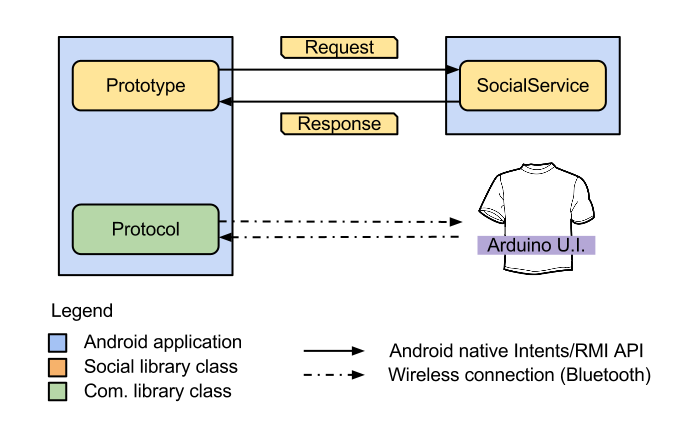
\includegraphics[scale=0.55]{img/design-toplevel.png}
	\caption{System architecture overview}
	\label{fig:design-toplevel}
\end{figure}


\section{System design}
\label{sec:system-design}
As the requirements for the product were not set early on by the customer, a lot of effort
was put into producing working prototypes to show during the meetings in order to receive
as much feedback as possible and identify the ideas the customer had in mind; these would provide
what was needed to proceed with system design. At some point, after roughly one month,
we understood that we were going in the wrong direction, and that our design wouldn't satisfy
the requirements the customer had mentioned. The design of some parts of the system had to be revised.

\subsection{First design}
Our first system design was based on the scenario where the user would download the T-shirt
and the social applications, browse for some content from within the social application
and actively send it to the tangible user interface (the T-shirt) by pressing a 'share' button.
This scenario is illustrated in figure \ref{fig:design-usecase1}.

\begin{figure}[h!]
	\centering 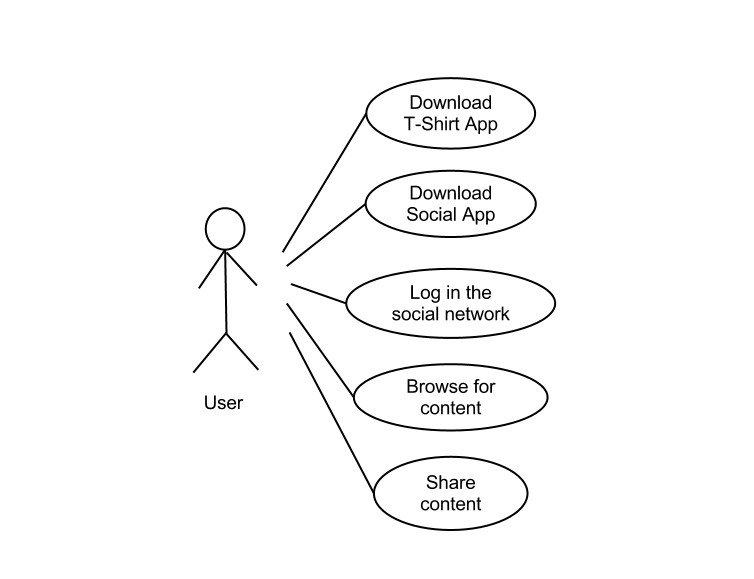
\includegraphics[scale=0.35]{img/design-usecase1}
	\caption{Use case for the product (first design)}
	\label{fig:design-usecase1}
\end{figure}

Please note that in this scenario the user is required to actively send data from
the social application (which acts as a Facebook client) to the T-shirt application,
which is merely capable of receiving. Also, both are implemented as Android applications.

The figure \ref{fig:design-resp} illustrates the communication between the applications.

\begin{figure}[h!]
	\centering 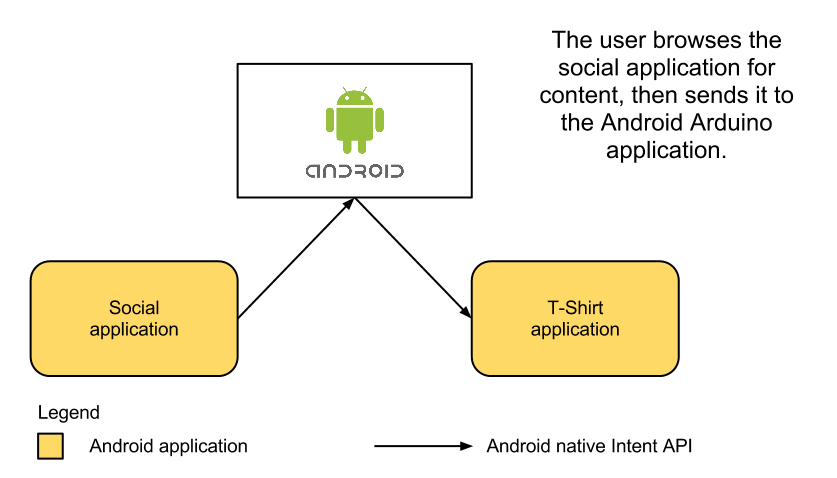
\includegraphics[scale=0.35]{img/design-resp.png}
	\caption{Communication diagram (first design)}
	\label{fig:design-resp}
\end{figure}


\subsection{Second design}
It turned out that the user was not supposed to browse for social content and actively send it 
to the T-shirt application. Instead, after downloading the software, he would just setup a set of rules
specifying the behavior of the T-shirt. This scenario is illustrated in figure \ref{fig:design-usecase2}

\begin{figure}[h!]
	\centering 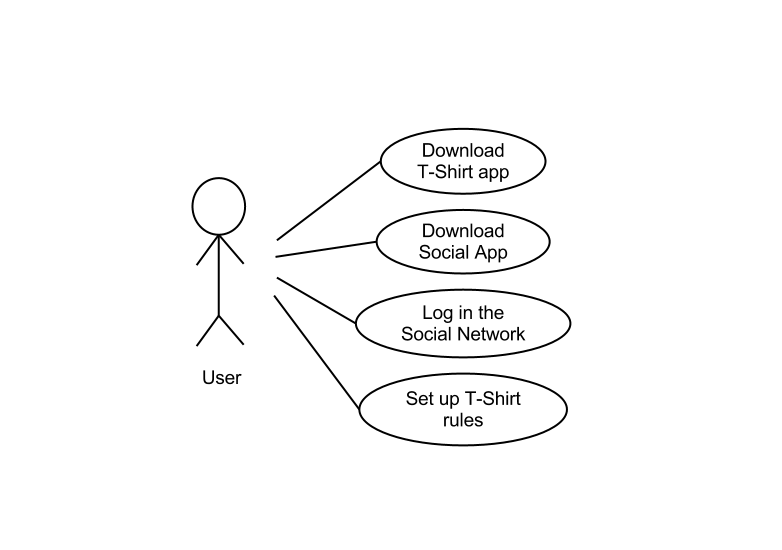
\includegraphics[scale=0.35]{img/design-usecase2}
	\caption{Use case for the product (second design)}
	\label{fig:design-usecase2}
\end{figure}

This new scenario made clear that the T-shirt and social applications had to be re-designed so:

\begin{itemize}

	\item [T-shirt application] A user interface, implemented as an Android application,
	that the user would to setup the rules for the T-shirt. The application needed also a
	background component (such as an Android service or Thread) that would 'ask' the required information
	to the social service.

	\item [Social application] An Android service that would run in the background, without user interaction,
	to fetch data from the social networks and return it to the T-shirt application.
	The service should also have a user interface in order to let the user authenticate and
	enable/disable the service itself.

	\end{itemize}

It also implied that a mechanism to request and exchange social content, as well as the necessary
data models abstractions had to be provided by the Social library. The figure \ref{fig:design-reqresp}
illustrates the communication between the services and the applications.

\begin{figure}[h!]
	\centering 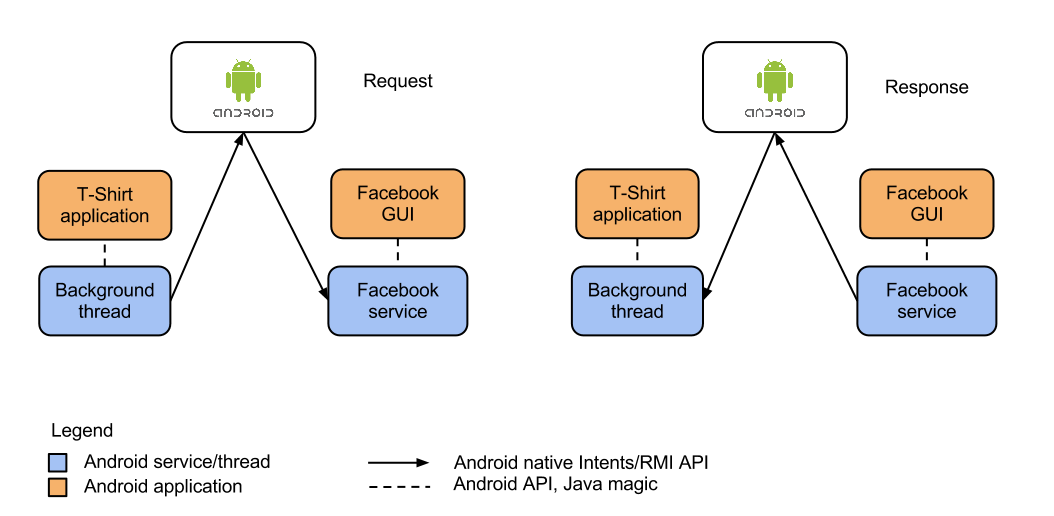
\includegraphics[scale=0.35]{img/design-reqresp.png}
	\caption{Communication diagram (second design)}
	\label{fig:design-reqresp}
\end{figure}

The T-shirt service is now 'asking' the social service for a specific content.
This happens in the background, without user interaction.

\subsubsection{Sequence diagram}
This sequence diagram show in figure \ref{fig:design-sequence} shows a sample communication between the social and T-shirt applications.
The T-shirt application requests the list of friends from Facebook whose age is the same as 'Anna'.

\begin{figure}[h!]
	\centering 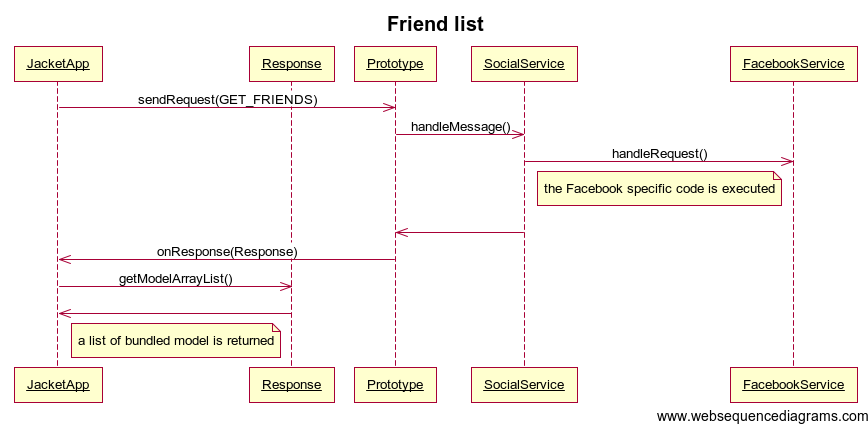
\includegraphics[width=1.0\textwidth]{img/design-sequence.png}
	\caption{Sequence diagram}
	\label{fig:design-sequence}
\end{figure}


\section{Libraries}

\subsection{The social library}
This library provides abstractions for many common concepts found in different
social networks like Facebook, Twitter and OpenSocial. This is done so that the developers
have the possibility to use these concepts seamlessly between any network and extend them to
possibily support others. It also defines and implements a sort of 'protocol' to allow Android
applications and services to exchange social data. This mechanism is based on Android's' native
inter-process communication API.

\todo {
	just cut one the 'first approach'?
}

\subsubsection{First approach}
Our first design approach consisted in a library that would handle the connection to social networks
such as Facebook, Twitter, LinkedIn, etc. This would allow the developers to write full-fledged
social 'multi-network' clients. It would also provide abstractions for common concepts
found in these networks such as Post, User, Comment and so on.

\subsubsection{Revised approach}
The big difference in the new approach is that the Social library won't provide any means
of connecting to social networks. Instead it will focus on establishing a communication interface,
using Android's inter-process communication, between Social applications and the Android-Arduino applications
to allow the exchange of social data. It will still provide abstractions for common concepts
found in social networks. This revised approach was made necessary after the first meetings with the customer
as we misunderstood the project scope, and went on to solve a very ambitious and unneeded task.
Some of the code and documentation we produced for the previous design was re-used, but some could not.

\todo {
	a class diagram maybe?
}


\subsection{The Communication library}
This library consists of a Java library (implemented on Android) and an Arduino firmware (figure \ref{fig:comlib-diagram}),
both implementing the ComLib protocol. The Java library provides a set of classes that simplify the connection to Arduino
devices that run the Communication library Arduino firmware. The library also implements a mechanism to request a list of 
services the remote device supports and any software download links associated with the remote device. A service might
be a sensor, a lamp, display screen while download links are represented as an URI link. All this meta information is stored
on in the firmware on the remote device as raw text using the JSON format. This meta-data can also be stored an retrieved
in a QR code or anything else that can store plain text.

\begin{figure}[h!]
	\centering 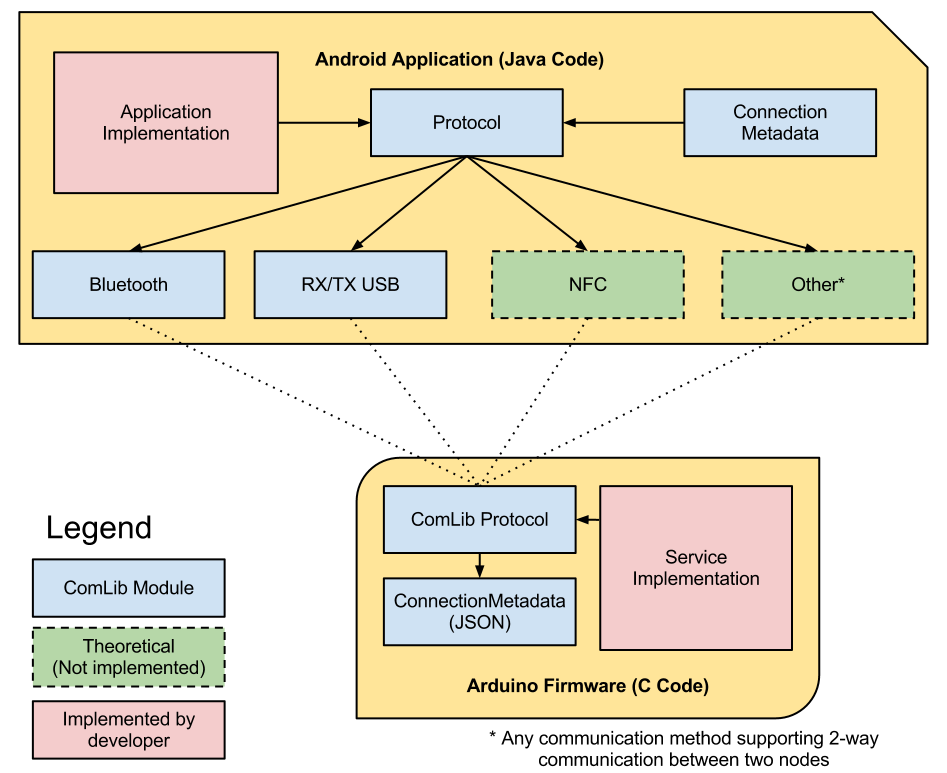
\includegraphics[scale=0.4]{img/comlib-diagram.png}
	\caption{Diagram for the Communication Library design}
	\label{fig:comlib-diagram}
\end{figure}

\subsubsection{The ComLib protocol}
The protocol is a basic set of rules that define how devices can communicate to the Arduino.
The ComLib protocol itself was designed by us, and has seen much changes in terms of which instructions were to be included,
and how the communication was to be executed. With the current design the Arduino cannot initiate the communication,
but is instead a passive device. For all instructions sent by any device to the Arduino, the Arduino sends a response,
either to acknowledge that it is finished executing the corresponding tasks, or the actually return the required
information in the "Content" field. An overview of the current instructions in the protocol can be seen in Table~\ref{tbl:opcodes}.

\begin{table}[h!]
	\begin{tabular}{ | c | c | p{1.5cm} | p{1.7cm} | p{6cm} |}
		\hline
		\textbf{Name} & \textbf{OPCODE} & \textbf{Flag} & \textbf{Content} & \textbf{Description} \\
		\hline
		Ping & 0x00 & N/A & N/A & Pings the arduino, to check that it's there \\
		\hline
		Text & 0x01 & N/A & Text to send & Sends text to the arduino, which then displays it depending on the implementation on the ardunio \\
		\hline
		Sensor & 0x02 & Sensor number & N/A & Requests sensor information from the arduino \\
		\hline
		Pin pulse & 0x03 & Pin number & N/A & Sends a 500ms pulse on the specified pin \\
		\hline
		Pin read & 0x04 & Pin number & N/A & Reads the current digital state of the specified pin on the arduino \\
		\hline
		Pin write & 0x05 & Pin number & Pin value (0 or 1) & Writes a digital state of a pin on the arduino \\
		\hline
		Response & 0xFE & Opcode & Response content & A response to a previous instruction, where the flag is the opcode for which it is the response to \\
		\hline
		Reset & 0xFF & N/A & N/A & Resets the arduino \\
		\hline
	\end{tabular}
	\caption{Overview of protocol's instructions}
	\label{tbl:opcodes}
\end{table}

\subsubsection{Arduino firmware implementation}
On the Arduino, all code related to our protocol is abstracted into a ComputerSerial library.
This library is a very basic state machine which processes single bytes received (see Figure~\ref{fig:arduino_states}).
The user of this library can register local methods to be called with RPC when the corresponding instruction is called.
The instructions follow strict rules on how they are constructed (see Table~\ref{tbl:instr_struct} for sizes of the different parts).
Each instruction has to start with a "start-byte" which is always 0xFF. The next part is the size, which tells the number of bytes
to come for this instruction (including the size byte itself). The rest is defined from which instruction is sent, but it is important to
remember that the content cannot be empty, and has to at least contain 1 byte. This byte however, is not necessarily read or used.

The following figure illustrates the Arduino automata.

\begin{figure}[h!]
	\centering
	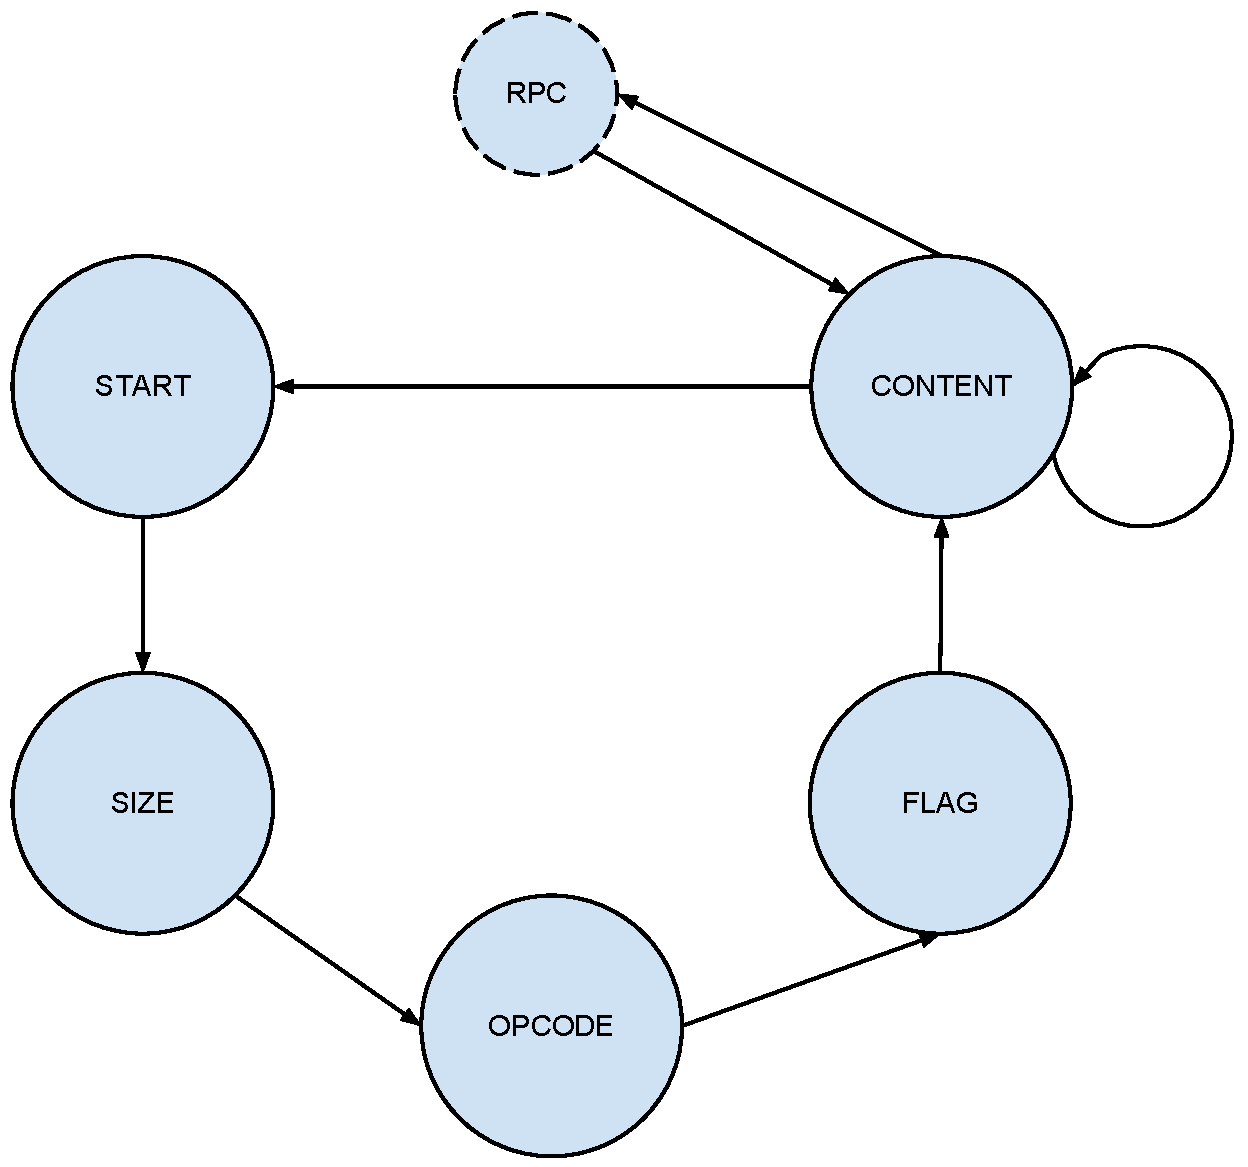
\includegraphics[width=\textwidth, keepaspectratio]{img/arduino_state-machine.pdf}
	\caption{The Arduino state-machine}
	\label{fig:arduino_states}
\end{figure}

\begin{table}
	\begin{tabular}{c|c|c|c|c|c|}
		\cline{2-6}
		& \textbf{Start-byte} & \textbf{Size} & \textbf{Opcode} & \textbf{Flag} & \textbf{Content} \\
		\hline
		\multicolumn{1}{|c|}{\textbf{Size}} & 1 & 1 & 1 & 1 & 1-252 \\
		\hline
	\end{tabular}
	\caption{Byte-structure of instructions}
	\label{tbl:instr_struct}
\end{table}


\section{Applications and Services}

\subsection{oSNAP application}

\subsection{T-shirt application}

As discussed in chapter \ref{sec:system-design} the T-shirt application design had to be reviewed after roughly one month.

\begin{figure}[h!]
	\centering 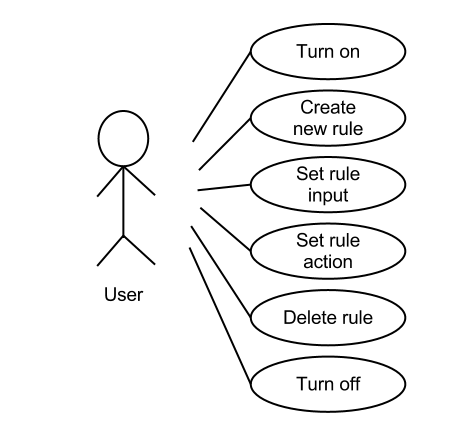
\includegraphics[scale=0.35]{img/design-tshirtappusecase2}
	\caption{Use case for the T-shirt application}
	\label{fig:design-tshirtappusecase2}
\end{figure}

For completeness we present the previous application use case in figure \ref{fig:design-tshirtappusecase1}

\begin{figure}[h!]
	\centering 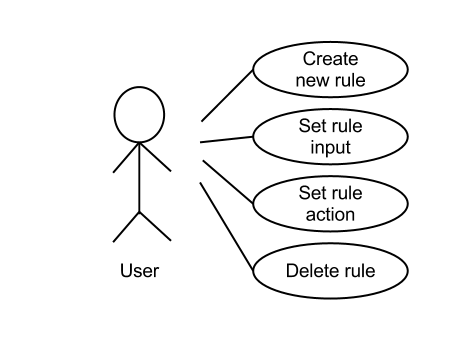
\includegraphics[scale=0.35]{img/design-tshirtappusecase1}
	\caption{Initial use case for the T-shirt application}
	\label{fig:design-tshirtappusecase1}
\end{figure}

\subsection{Facebook application}

As discussed in chapter \ref{sec:system-design} the Facebook application design had to be reviewed after roughly one month.

\begin{figure}[h!]
	\centering 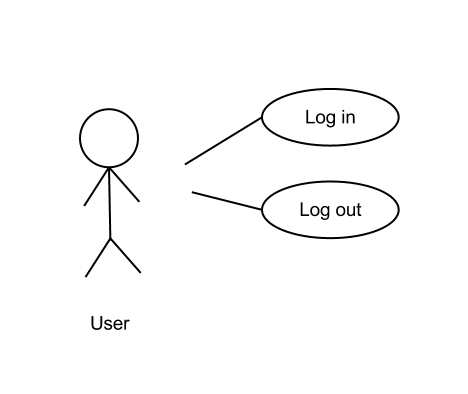
\includegraphics[scale=0.35]{img/design-socialappusecase2}
	\caption{Use case for the Social application}
	\label{fig:design-socialappusecase2}
\end{figure}

For completeness we present the previous application use case in figure \ref{fig:design-socialappusecase1}.

\begin{figure}[h!]
	\centering 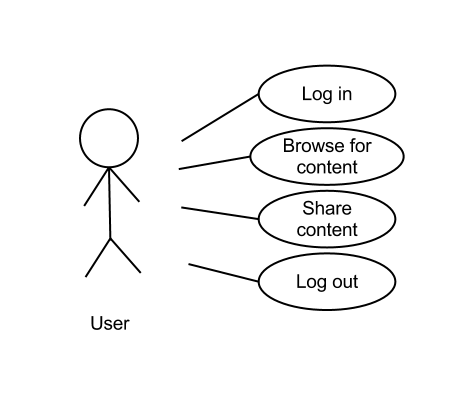
\includegraphics[scale=0.35]{img/design-socialappusecase1}
	\caption{Initial use case for the Social application}
	\label{fig:design-socialappusecase1}
\end{figure}

\subsection{Twitter application}
\subsection{Temperature application}
\subsection{LED matrix application}


\section{Prototypes}
\label{sec:prototypes}
Three different prototypes will be produced for the project. Their purpose is to serve as proof of concept and
to show that the libraries and can effectively simplify the prototyping of Arduino-based T.U.I.
One of the prototypes, the T-shirt, is significantly bigger and more complex than the other two.
The T-shirt is the main prototype of the project; the purpose of the other two
is just to show that the libraries can be use for other applications and in different contexts.

\subsection{Prototype 1: The social Jacket}
	
\begin{figure}
	\begin{center}
	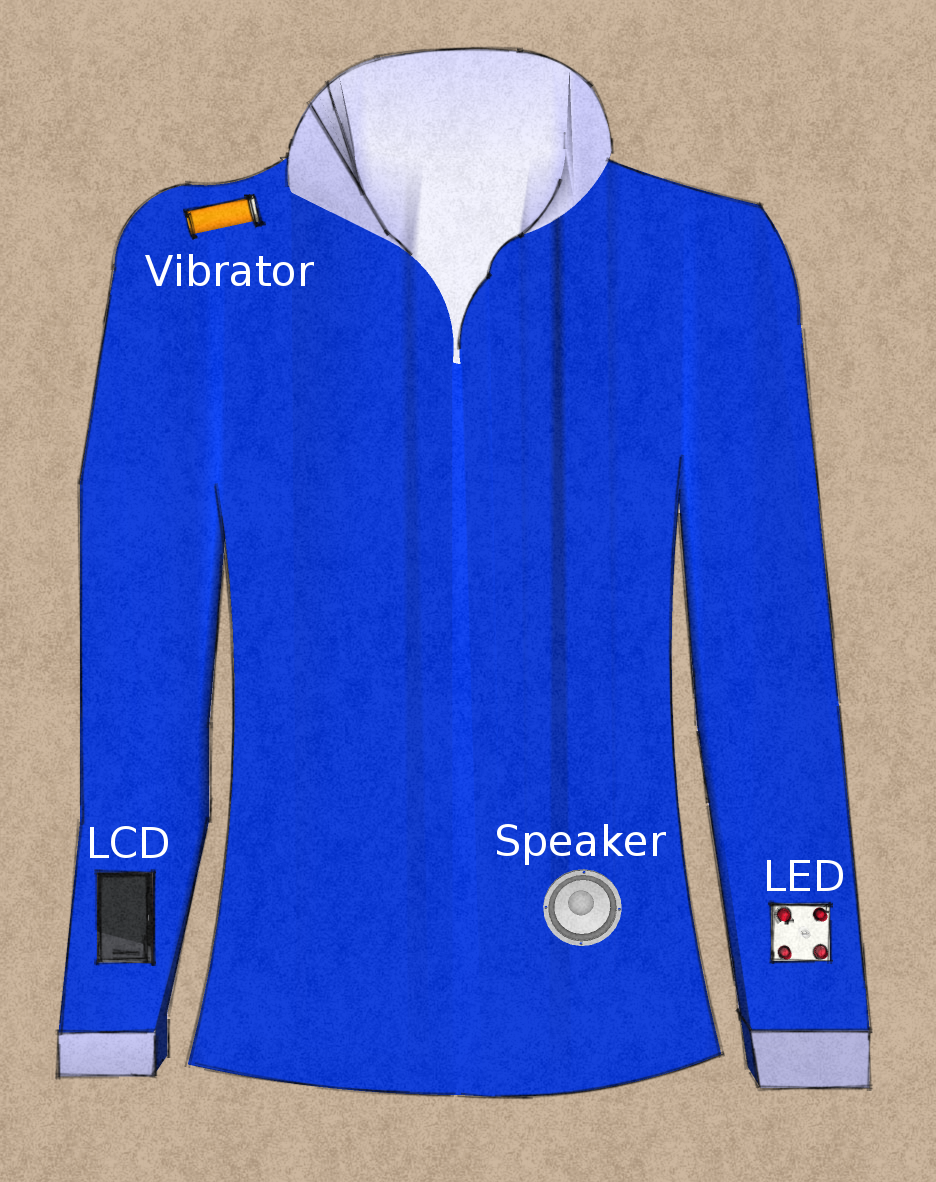
\includegraphics[scale=0.2]{img/design-tshirtproto}
	\end{center}
	\caption{Concept drawing of the Jacket Prototype}
	\label{fig:design-TShirt}
\end{figure}
	
This is our main prototype and will showcase a lot features.
It consists of aJacket connected to a Lilypad Arduino that will feature
several displays and indicators which will receive social data from an Android phone.
The shirt features different tangible interfaces (see figure \ref{fig:design-TShirt}):
	
\begin{itemize}
	\item LEDs
	\item LCD Display
	\item Sound speaker
	\item Vibration module
\end{itemize}
	
Any of these can be mapped to a fair deal of concepts found in social network.
So a "Poke" from Facebook could become a vibration on the Jacket. When someone "Likes" your post a small sound effect
could be played, a LED blinking on status updates from Twitter, etc. The Jacket is connected to the social networks
through a wireless connection to an Android mobile. Specifically, the mobile Android is connected to the Internet
and carried in the pocket of the person using the Jacket and is connected wirelessly with the Arduino Lilypad through Bluetooth.

	
\subsection{Prototype 2: Temperature Sensor for Android}
This prototype will primarily showcase the communication from Arduino to Android using our libraries. 
Figure \ref{fig:design-temperature} shows a visual representation of the entire Temperature Sensor
prototype with an Android device connected wirelessy through bluetooth to the Arduino board. The 
Arduino unit can read the ambient temperature and be able to send this info to an Android application,
 either on demand or at a set interval that can be chosen through settings in the application. 
In the planning stage of this prototype, a paper prototype (see figure~\ref{fig:prototype2-paper}) was showed to the
customer. Due to some problems with getting the initial design to work properly, the GUI was revised(see
figure~\ref{fig:prototype2-gui} ) to make it more user friendly and visually appealing.

\begin{figure}[H]
	\centering
	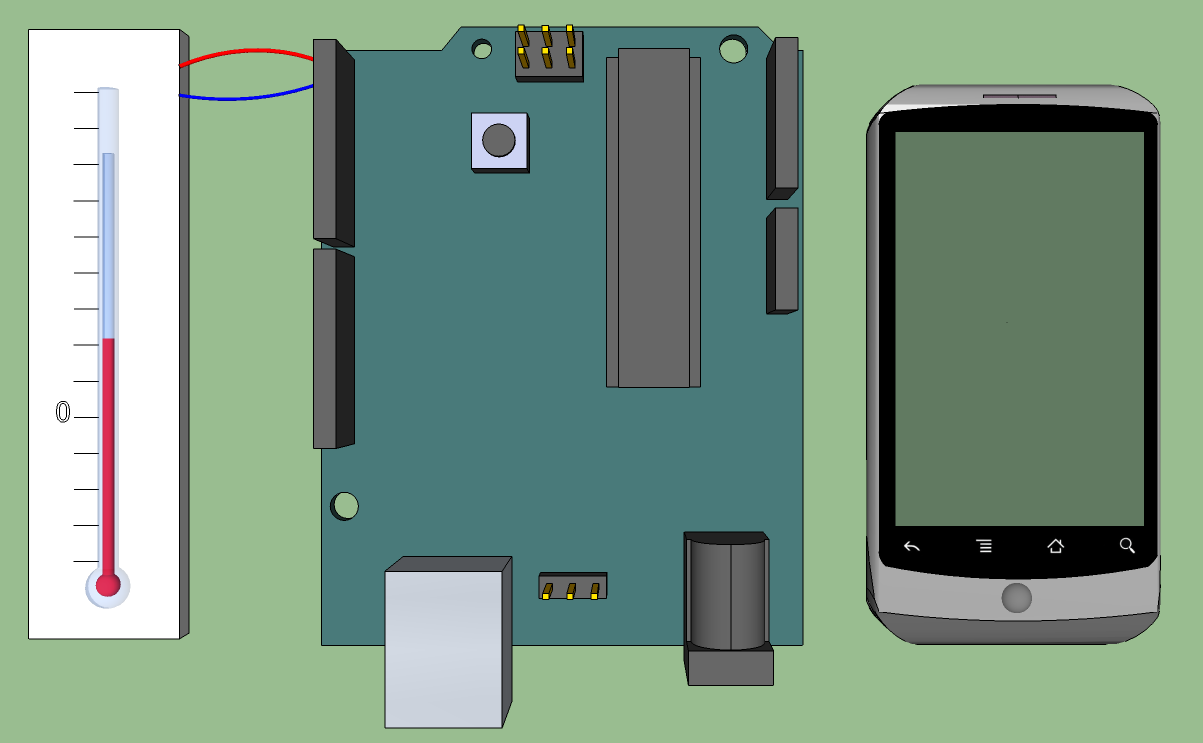
\includegraphics[scale=0.35]{img/design-temperature}
	\caption{Concept drawing of the temperature application setup.}
	\label{fig:design-temperature}
\end{figure}

\begin{figure}[H]
\centering 
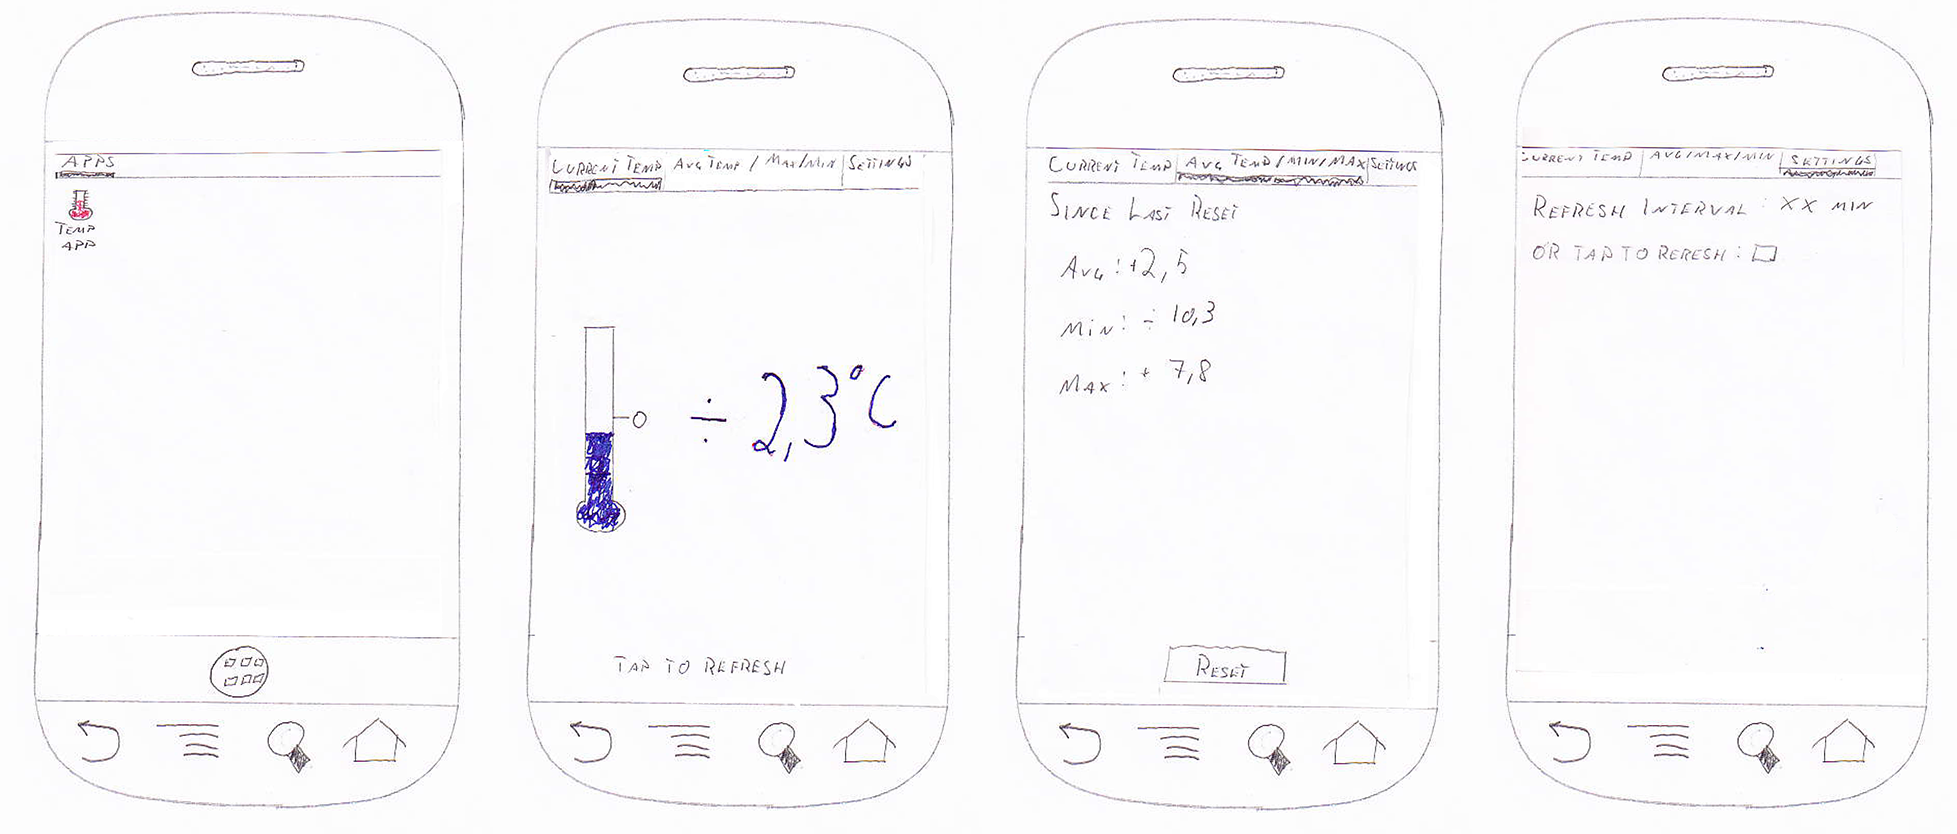
\includegraphics[width=1.0\textwidth]{img/prototype2-paper.png}
\caption{Paperprototype for the temperature sensor.}
\label{fig:prototype2-paper}
\end{figure}

\begin{figure}[H]
\centering 
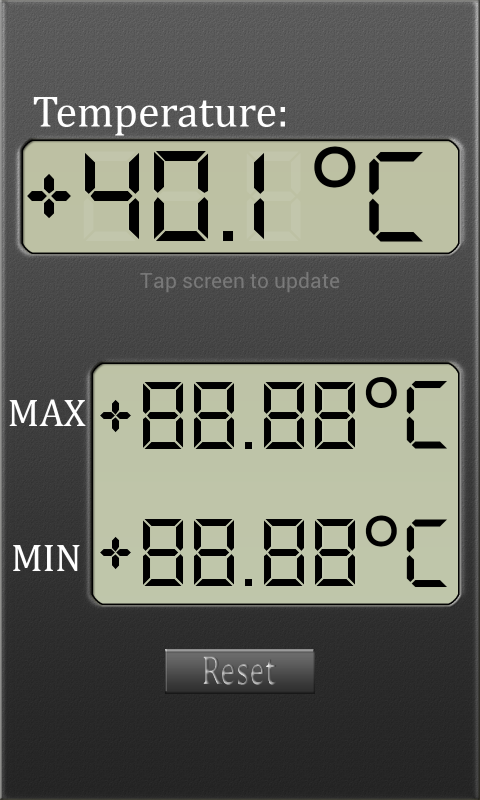
\includegraphics[width=0.3\textwidth]{img/prototype2-gui.png}
\caption{Final GUI design for the temperature prototype.}
\label{fig:prototype2-gui}
\end{figure}

	
\subsection{Prototype 3: Wearable Pictures}
This prototype was first planned to be LED lights (Figure \ref{fig:design-ledmatrix}) showing what mood you had on MySpace.
Red LED lights would be angry, green would be happy and so on. We discovered that MySpace had removed this feature from their pages,
even if it was still supported by the API. It would be a fools errand to pursue something you could not test properly
in a real world situation, so we changed the concept of this prototype. It ended up to be a sort of wearable fashion.
You select colors of the 3x3 LEDS in a graphical interface in an Android app. Then you send this information over Bluetooth
to the Arduino who shows the selected colors on a necklace.

\begin{figure}
	\begin{center}
	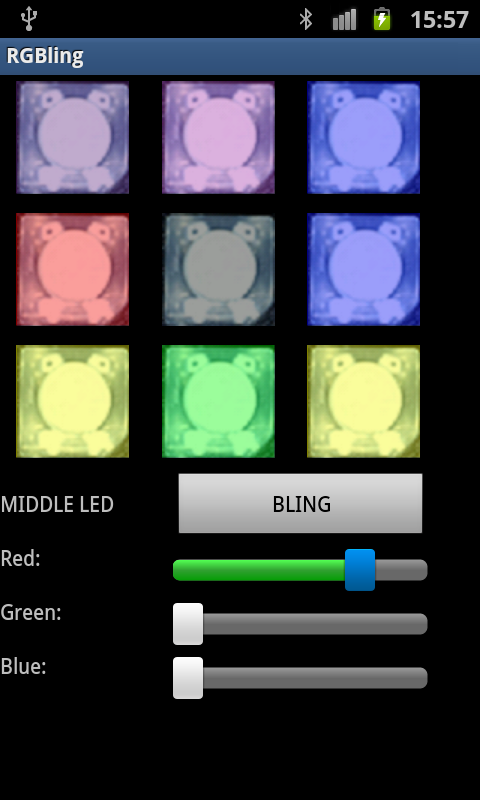
\includegraphics[scale=0.7]{img/prototype3rgBling.png}
	\end{center}
	\caption{Concept of the Android application RGBling.}
	\label{fig:design-ledmatrix}
\end{figure}

\section{Package Structure}
The source code of the whole system can be organized in smaller sections.
Here we describes some of the packages we have divided the system code into.
The system was coded in Arduino C and Java. Java was used to code Android libraries and applications.
Arduino C code is executed on the Arduino board. The Java code is again divided into packages.
Below is a brief description of the most important ones.

\subsection{Java code}
\begin{itemize}
	\item \textbf{no.ntnu.osnap.com}\newline
		Communication Library contains every class to establish a connection with a remote device using a general
		protocol interface. The actual details of the communication such as Bluetooth, cable, WiFi, stream-based or
		sockets are hidden away from the user. This is to provide a simple and generic interface to all supported
		communication methods. The user can easily add new communication types by extending an abstract class.
		The ComLib additionally defines a standard of storing and retrieving meta-data of services and download URI
		links from the remote device using JSON.
	\item \textbf{no.ntnu.osnap.com.testing}\newline
		Test units and sample programs for the ComLib. These are simple test applications that are run on
		the Android to test if the ComLib is communication correctly using the specified
		protocol.
	\item \textbf{no.ntnu.osnap.social}\newline
		Social library main classes.
	\item \textbf{no.ntnu.osnap.models}\newline
		Social library data models.
	\item \textbf{no.ntnu.osnap.listeners}\newline
		Social library listeners.
	\item \textbf{no.ntnu.osnap.tshirt}\newline
		T-shirt application classes.
	\item \textbf{no.ntnu.osnap.temp}\newline
		Temperature application classes.
	\item \textbf{no.ntnu.osnap.led}\newline
		Led application classes.
	\item \textbf{no.ntnu.osnap.mockups}  \newline
		Stubs and 'driver' applications used for testing purposes.
		Example applications for third-party developers.
\end{itemize}

\subsection{Arduino C code}
All the Arduino code is in one class, and there is therefore no package structure to speak of.
The class consists of a header file and a source file. This is then to be included in Arduino projects
that want to use our protocol for communication.


\subsection{Hardware}

\todo {
	schematics? Pics of Arduino boards, thoughs.
}
